\chapter{Simulación de tráfico}
\label{ch:sota-traffic-simulation}

El tráfico es un sistema caótico en el que intervienen un número muy elevado de diferentes variables, muchas de las cuales relacionadas entre si. Debido a esto, obtener modelos exactos de tráfico es una tarea prácticamente imposible y es por ello que la mayoría del trabajo cuyo objetivo es la predicción se realice en base a simuladores.

Los simuladores de tráfico son herramientas de software que, usando diferentes modelos, describen el tráfico como sistema, permitiendo:

\begin{itemize}
	\item Extraer resultados y conclusiones de escenarios de tráfico determinados.
	\item Implementar técnicas de tráfico sin necesidad de alterar el tráfico real.
	\item Reproducir exactamente un escenario.
	\item Introducir modificaciones en puntos determinados (e.g. espaciales o temoprales) de un escenario conocido para evaluar la divergencia en su evolución.
\end{itemize}

Los objetivos en la simulación de tráfico son los de hacer que los modelos se parezcan lo máximo posible a la realidad. En este capítulo vamos a ver cuál es la realidad actual de este tipo de simuladores, cuáles son sus diferentes tipologías y maneras de modelar los diferentes aspectos del tráfico y, posteriormente, realizaremos una evaluación de cuáles son los idóneos para nuestro trabajo.

Limitaremos el estudio no obstante a los simuladores de vehículos, obviando otros tipos de simulación de tráfico que no tienen que ver con esta temática, como por ejemplo los orientados a la evaluación de sistemas de señalización inteligentes (e.g.~\cite{jin2016evaluation}) o a la estimación de emisiones (e.g.~\cite{quaassdorff2016microscale}).

\section{Clasificación de simuladores de tráfico}

Los aspectos simulables y medibles del problema tráfico son muy diversos, dependiendo sobre todo del nivel de complejidad del tráfico\sidenote{Modelar una vía por la que circula un centenar de coches no es lo mismo que modelar una ciudad donde circulan millones.}, de qué queremos medir\sidenote{Evaluar a un conductor en una situación determinada o evaluar la evolución del flujo de tráfico en un cuello de botella causado por un accidente.} y de cómo lo modelamos\sidenote{Un autómata celular se modela de forma diferente a un modelo lineal de vías o carriles.}.

El resto de la sección ofrece una visión de las diferentes categorías en las que se clasifican los simuladores de tráfico.

\subsection{Tipos de simulador en función de la complejidad}

La complejidad en una simulación se refiere al nivel de detalle al que queremos llegar a la hora de modelar nuestra solución. Es evidente que según aumentamos el detalle en la simulación aumenta la cantidad de cálculo. Por ejemplo, si queremos modelar el comportamiento de $10$ billones de canicas cayendo por un tubo es considerablemente más eficiente modelarlas como un fluido con una serie de propiedades características que como una colección de elementos individuales, cada uno con sus propiedades (e.g. masa, aceleración, ...) e interaccionando entre sí.

\begin{figure}
	\centering
	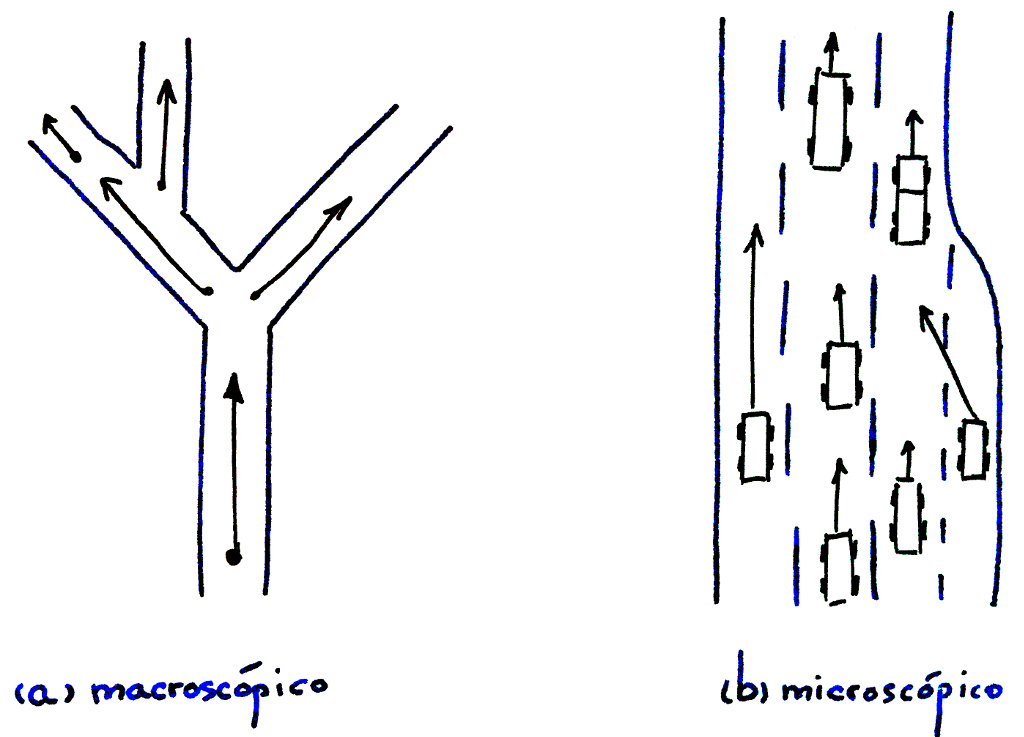
\includegraphics{images/granularities-in-traffic-simulation}
	\caption{Taxonomía clásica de los simuladores en función de la granularidad (complejidad) de la simulación.}
	\label{fig:granularities-in-traffic-simulation}
\end{figure}

En el caso de los simuladores de tráfico es lo mismo. En éstos existe un amplio intervalo de granularidades, desde por ejemplo el flujo de entrada en una autovía hasta el consumo de carburante de un vehículo en ciudad. Lo más común es clasificar los simuladores dentro de dos grandes grupos, los cuales se ilustran en la Figura~\ref{fig:granularities-in-traffic-simulation}:

\begin{itemize}
	\item \textbf{Microsimulación} o simulación de tipo \textbf{micro}. Su objetivo es estudiar, desde un punto de vista de granularidad fina como puede ser vehículos o peatones, las micropropiedades del flujo de tráfico como, por ejemplo, los cambios de carril, las aproximaciones a vehículos delanteros o los adelantamientos, para evaluar su comportamiento. Tiene dos principales ventajas, la posibilidad de estudiar el tráfico como un todo a partir de sus elementos más simples (ofreciendo una representación más fiel de éste) y la posibilidad de estudiar cada elemento por separado. Sin embargo, la principal desventaja de este tipo de modelos es que cada elemento de la simulación requiere de cómputo independiente y por tanto simulaciones con alto contenido de elementos pueden llegar a ser inviables\sidenote{Existen técnicas de computación distribuida que superan ampliamente los límites impuestos por la computación en un único nodo, por ejemplo, el simulador de IBM \textit{Megaffic}. Éste implementa un modelo de granularidad micro donde cada elemento es un agente independiente (i.e. sistema multiagente) usando para ello entornos con cientos de núcleos de proceso que proveen de capacidad suficiente para modelar ciudades enteras como Tokio (ver~\cite{Osogami2012} y~\cite{Suzumura2012}).}.
	\item \textbf{Macrosimulación} o simulación de tipo \textbf{macro}. Este tipo de modelos centran su esfuerzo en estudiar el flujo de tráfico como un todo, explorando sus macropropiedades (e.g. evolución del tráfico, efectos onda, velocidad media o flujo en vías). Su ventaja principal es que a nivel macroscópico permiten estudiar propiedades que a nivel microscópico requeriría una cantidad ingente de recursos. Sin embargo, con este modelo es imposible obtener información precisa de un elemento en particular del tráfico.
\end{itemize}

Aunque esta es la categorización típica de modelos, en la literatura aparecen otros tipos de modelo con granularidades que pueden considerarse no pertenecientes a ninguno de estos dos conjuntos. Este es el caso de los simuladores de tipos \textbf{sub-micro} y los \textbf{meso} (ver figura~\ref{fig:mesoscopic-and-submicroscopic-simulation}). 

\begin{figure}
	\centering
	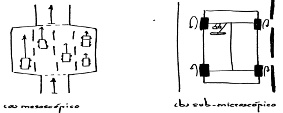
\includegraphics{images/mesoscopic-and-submicroscopic-simulation}
	\caption{Aproximaciones alternativas de modelos en función de la complejidad. Ejemplo de mesosimulación como ventana de microsimulación dentro de un flujo en un macrosimulador (e.g. \cite{munoz2001integrated}) y ejemplo de submicrosimulación donde se modelan componentes internos del vehículo.}
	\label{fig:mesoscopic-and-submicroscopic-simulation}
\end{figure}

Los \textbf{sub-micromodelos} especifican granularidades por debajo del nivel de \enquote{vehículo} o \enquote{peatón}. Por ejemplo, en (\cite{Minderhoud1999}) trabaja a nivel de funcionamiento del control de crucero inteligente de un vehículo en función del entorno del vehículo.

Por otro lado los \textbf{mesosimuladores} (e.g.~\cite{munoz2001integrated} o~\cite{casas2011need}) nacen para amortiguar los problemas inherentes a la complejidad en los micromodelos y a la falta de resolución en los macromodelos.

Dado que en nuestro discurso trabajaremos en la evaluación de modelos de comportamiento de conductores, nos ceñiremos al uso de simuladores que modelen un nivel de granularidad \textbf{micro}.

\subsection{Tipos de simulador en función del espacio y el tiempo}

Existen otras dos formas de clasificar los simuladores en función de cómo evolucionan en la simulación el \textbf{tiempo} y el \textbf{espacio}. Sin embargo, aunque \textit{complejidad}, \textit{tiempo} y \textit{espacio} son dimensiones diferentes a la hora de clasificar simuladores, el tipo de simulador según complejidad determina en gran medida los tipos según las dimensiones espacio y tiempo.

\begin{figure}
	\centering
	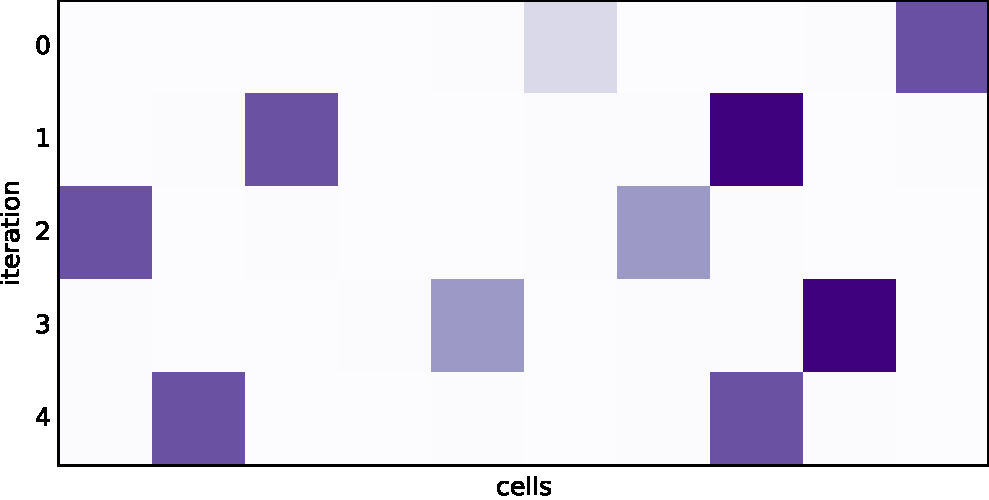
\includegraphics[width=.8\linewidth]{images/cellular-automata-based-sim}
	\caption{Ejemplo de un simulador de tráfico basado en autómatas celulares. En éste, el espacio se divide en celdas que pueden, o bien estar vacías, o bien ocupadas por un vehículo. La ilustración representa la evolución de los tiempos para cada vehículo (representado por un punto) según se desplaza a través del espacio discertizado en celdas de $7.5m$. Concretamente muestra la evolución a lo largo del tiempo del movimiento de un modelo de \textit{car-following} de tres vehículos. Fuente:~\cite{Brilon1999}.}
	\label{fig:cellular-automata-based-sim}
\end{figure}

En el caso del espacio, la clasificación diferencia las simulaciones que se mueven por un espacio discreto o por uno continuo:

\begin{itemize}
	\item De espacio \textbf{discreto}. Simulación donde el espacio está dividido en celdas que nosmalmente sólo pueden estar ocupadas por un elemento en un momento determinado. Este es el caso, por ejemplo, de los simuladores basados en autómatas celulares. La figura~\ref{fig:cellular-automata-based-sim} ilustra el comportamiento de uno de estos tipos de simulador.
	\item De espacio \textbf{continuo}. Simulación que transcurre en una secuencia infinita de puntos en el espacio. Es el caso por ejemplo de los simuladores basados en modelos lineales, como podemos ver en el ejemplo de la figura~\ref{fig:car-following-based-sim}.
\end{itemize}

En el caso del tiempo, la división se realiza en los mismos términos que en los del espacio:

\begin{itemize}
	\item De tiempo \textbf{discreto}. También denominada de \textit{simulación de eventos discretos}, divide el tiempo en intervalos discretos, generalmente (aunque existen excepciones) de longitud fija duranet toda la simulación. Los simuladores basados en autómatas celulares son también simuladores típicos discretos, ya que cada posición en el espacio se va calculando para cada intervalo discreto de tiempo (ver figuras~\ref{fig:cellular-automata-based-sim} y~\ref{fig:nagel-schreck}).
	\item De tiempo \textbf{continuo}. En estos simuladores el tiempo es un factor más para un modelo de ecuaciones diferenciales. La figura~\ref{fig:car-following-based-sim} ilustra un modelo de \textit{car-following} que puede implementarse en una smiulación de tiempo continuo si la aceleración viene determinada por un modelo que entre otros factores incluye el tiempo.
\end{itemize}

\begin{figure}
	\centering
	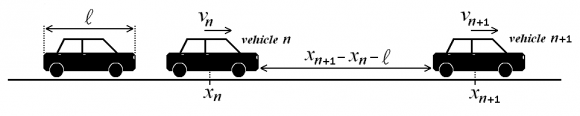
\includegraphics{images/car-following-based-sim}
	\caption{Ejemplo de un modelo lineal en un espacio continuo. La posición del vehículo es un valor $x \in \mathbb{R}$. Este ejemplo representa un modelo de \textit{car-following} donde el comportamiento de la aceleración del vehículo es determinado por la distancia al coche siguiente. Fuente:~\cite{Tordeux2011}.}
	\label{fig:car-following-based-sim}
\end{figure}

En nuestro caso, queremos conocer la situación exacta del vehículo y no una situación aproximada en una separación discreta del espacio. Esto nos dirige hacia simuladores de espacio continuo. Por otro lado, nosotros realizamos la recolección de datos en intervalos cuantificables de tiempo, los cuales serán usados para modelar los comportamientos de los conductores y para contrastar los resultados; por tanto, la elección está sesgada hacia simulación de tiempo discreto.

\section{Modelos de microsimulación}

En el caso concreto de la microsimulación, la literatura distingue entre tres diferentes aproximaciones a la hora de representar el tráfico. Éstas son la de autómatas celulares, al de sistemas de partículas y la de sistemas multiagentes.

\subsection{Microsimulación basada en autómatas celulares}

Un autómata celular es una colección ordenada de celdas o \textit{células} $n$-dimensionales que parcelan el universo en estudio. Cada una de dichas celdas se encuentra en un estado (e.g. contiene un valor numérico), y el estado de todas ellas se actualiza síncronamente (esto es, todas a la vez) en intervalos regulares de tiempo denominados \textit{ciclos}. El camio de estado de cada célula depende de los valores de las células vecinas y del algoritmo de modificación al que responden todas y cada una de las células.\sidenote{Hay realmente máquinas capaces de operar de esta manera, es decir, arquitecturas basadas en autómatas celulares. En ellas, cada ciclo de reloj actualiza todas las celdas de memoria del autómata. Éstas arquitecturas se suelen usar para la implementación de modelos físicos \TODO{buscar referencias}, superando en varios órdenes de magnitud la capacidad computacional de las arquitecturas tradicionales.}.

Estos modelos de microsimulación, debido a la propia naturaleza de los autómatas celulares, se encuentran clasificados como simuladores de tiempo y espacio discretos, y se usa debido a su facilidad de implementación y su eficiencia, ya que es fácilmente paralelizable.


\begin{figure}
	\centering
	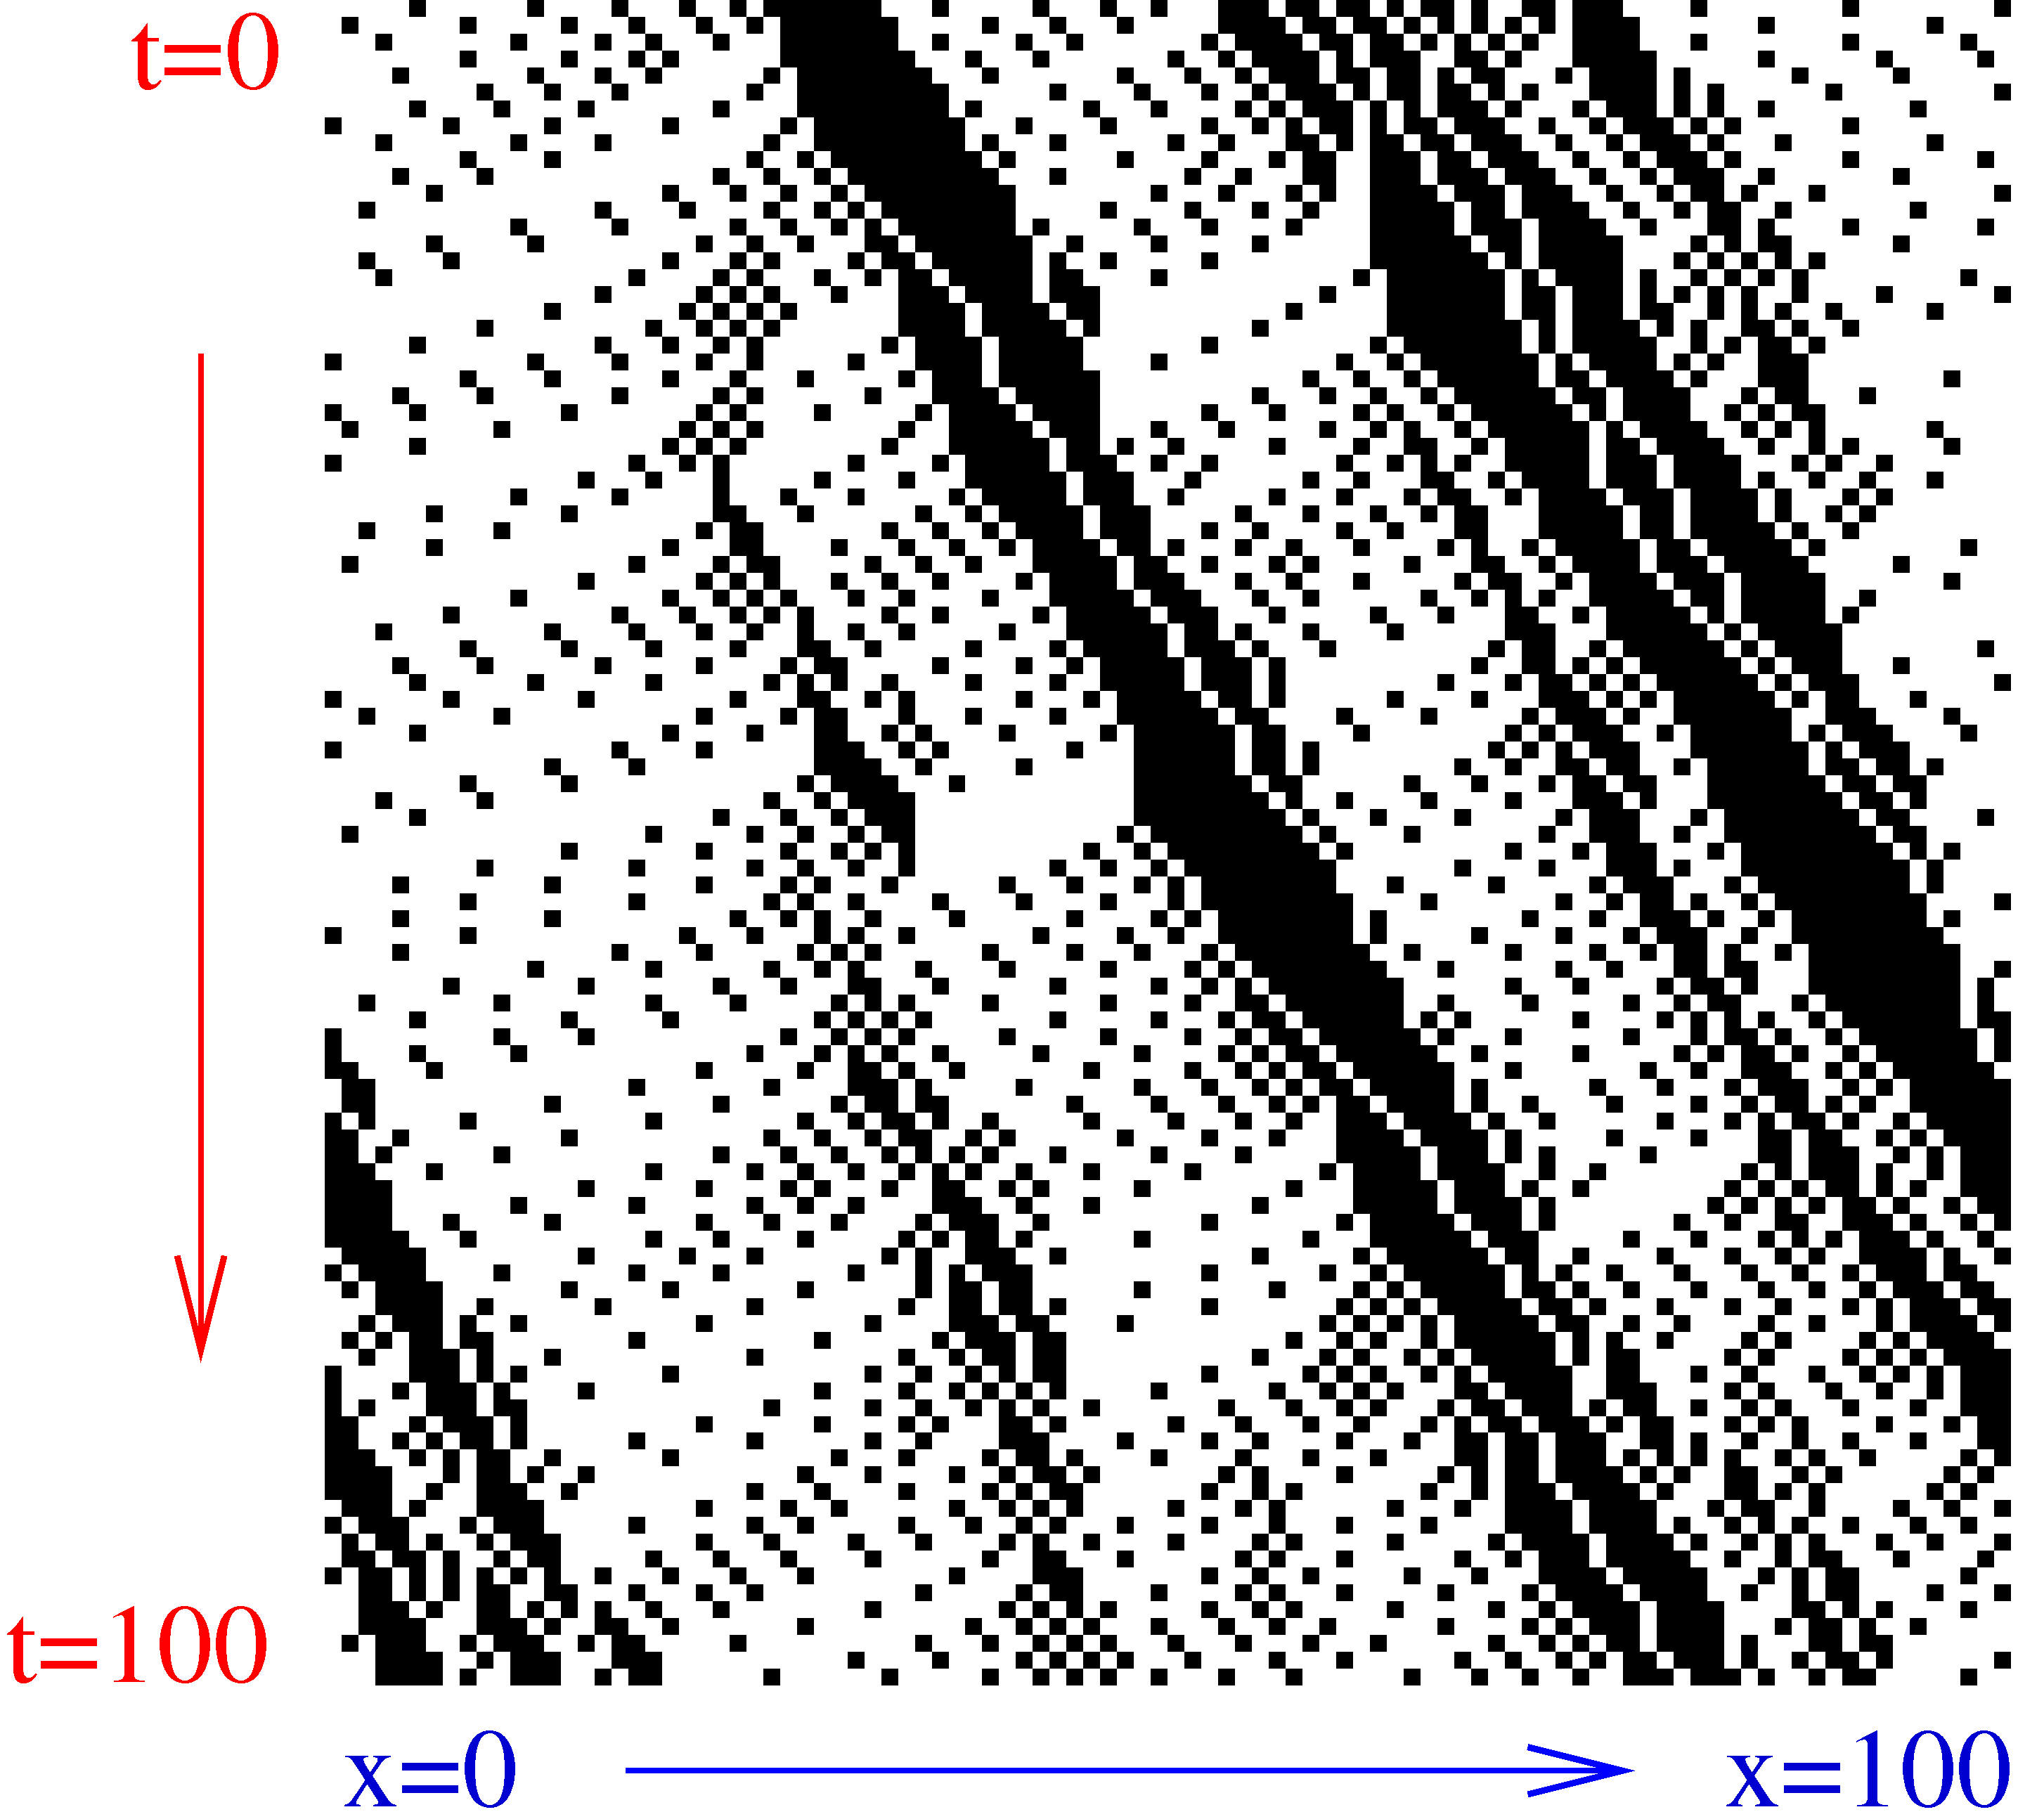
\includegraphics[width=.75\linewidth]{images/nagel-schreck}
	\caption{Representación de la evolución de un atasco en una autopista  de $100$ celdas de longitud usando el modelo Nagel-Scherckenberg. Con una densidad de ocupación $\rho = 0.35$ y una probabilidad de frenada de $p = 0.35$ se puede observar en la figura cómo se desplazan las olas del atasco a lo largo de los $100$ ciclos de la simulación. Feunte: Wikimedia}
	\label{fig:nagel-schreck}
\end{figure}

El modelo clásico de esta aproximación es el de Nagel-Scherckenberg (\cite{Nagel1992}), un modelo teórico creado para la simulación de tráfico en autopistas. La figura~\ref{fig:nagel-schreck} muestra la evolución del tráfico en una autopista a lo largo del tiempo de un autómata de este tipo. El resúmen de su funcionamiento es el siguiente:

\begin{itemize}
	\item La vía está divida en celdas de longitud $7,5m$ debido a que esta distancia es la media entre los parachoques traseros de dos coches consecutivos en un atasco.
	\item La celda puede tener dos estados, vacía o con un coche a una velocidad $v = \{0, \ldots, v_{max}\} \in \mathbb{N}$, esto es, discreta. La unidad de medida es $c/\Delta t$ siendo $c$ un número de celdas.
	\item $\Delta t$ queda establecido en $1s$, considerado el tiempo medio de reacción de un conductor ante una eventualidad. Esto hace, por ejemplo, que una velocidad de $6 c/\Delta t$ sea $45 m/s$ ($162 km/h$).
	\item En cada ciclo, se realizan cuatro acciones de manera simultánea: acelerar (nua unidad si no están a la máxmia velocidad), frenar (si se ven obligados en función de la velocidad y la distancia del siguiente vehículo), freno aleatorio (con una probabilidad de $p = 0.5$ la velocidad se reduce en una unidad hasta un mínimo de $v = 1 c/\Delta t$) y reposicionamiento (se avanzan tantas celdas como indica la velocidad.)
\end{itemize}

En general los modelos de la literatura suelen ser una variación de éste con ligeras modificaciones para estudiar aspectos concretos de modelos de tráfico, como la modificación del paso de \textit{aleatorización} (e.g. \cite{Barlovic1998}) o celdas más pequeñas (e.g. \cite{Krauss1997}) para comprobar la metaestabilidad del flujo de tráfico, o modelos y reglas para vías de dos carriles (e.g. \cite{Brilon1999} en la figura~\ref{fig:cellular-automata-based-sim} y~\cite{Nagel1998}).  se basan en éste lo amplían para superar algunas de sus limitaciones.

\subsection{Microsimulación basada en sistemas de partículas}

Dentro de la microsimulación, he visto que hay diferentes aproximaciones. Autómatas celulares, sistemas de partículas, sistemas multiagentes. Buscarmás y describir aquí. El caso es que por lo que veo, de esostres sólo nos interesan los mas. Explicarlos aquí.

\subsection{Microsimulación basada en sistemas multiagentes}

Dentro de la microsimulación, he visto que hay diferentes aproximaciones. Autómatas celulares, sistemas de partículas, sistemas multiagentes. Buscarmás y describir aquí. El caso es que por lo que veo, de esostres sólo nos interesan los mas. Explicarlos aquí.

\section{Elección de software para las simulaciones}

En este apartado se facilita la comparativa realizada para la elección de simulador sobre el que basar los escenarios a plantear en las simulaciones de los modelos de conductor.

Hoy en día existe una oferta muy amplia de simuladores en el mercado, cada uno implementando uno o varios modelos diferentes y bajo diferentes licencias.

Cada simulador tiene sus ventajas e inconvenientes, y es por ello importante realizar un estudio previo para conocerlos y no llevarse sorpresas una vez se llega a estadios más avanzados del estudio. No se trata de realizar una comparativa en busca del mejor simlador de tráfico del mercado, sino en encontrar el simulador que más se adecúa a los criterios concretos para los propósitos de esta tesis.

\subsection{Entornos de simulación a estudiar}

El siguiente listado muestra la lista de simuladores de tráfico sobre los que se realizarán las comparativas. Por motivos de espacio no se han incluido todos los simuladores encontrados en la listeratura, sino que se han seleccionado únicamente aquellos que (i) aun existen y se pueden adquirir, y (ii) son entornos de microsimulación.

\begin{enumerate}
	\item \textbf{AIMSUN}. Entorno de simulación de granularidad micro, meso y macro desarrollado por la empresa \textit{Transport Simulation Systems}. Url: \url{http://www.aimsun.com/}.
	\item \textbf{TSIS-CORSIM}. Entorno de microsimulación compuesto de dos simuladores para distintos modos de tráfico (NETSIM para entornos urbanos y FRESIM para entornos interurbanos) desarrollado dentro de la Universidad de Florida por el centro \textit{McTrans}. Url: \url{http://mctrans.ce.ufl.edu/featured/tsis/}.
\end{enumerate}

Simuladores de pago:

Quadstone paramics (microscopic)
VISSUM (macroscopic)
VISSIM (microscopic)
ARCHISIM

Simuladores gratuitos:

Matsim
SUMO (microscopic)
Repast
MAINSIM
Synchro

Ni puta idea:

CUBE
SATURN
PARAMICS
TRANSIMS


\subsection{Criterios de selección}

Los criterios se muestran ordenados alfabéticamente:

\begin{enumerate}
	\item \textbf{Activo}. Si el simulador está activaemnte desarrollado o si por el contrario se trata de un proyecto con poca actividad por parte de sus autores. Es interesante hacer uso de un simulador que esté siendo activamente desarrollado porque eso favorece la aparición de parches y mejoras sobre el software.
	\item \textbf{Extensibilidad}. Si el simulador permite extender sus funcionalidades de alguna manera. Aunque se puede considerar que si es Open Software, es posible modificar su comportamiento para adcuarlo a los modelos desarrollados, es mejor que el propio software ofrezca los mecanismos necesarios para la integración sin necesidad de tocar el núcleo.
	\item \textbf{Granularidad}. Si el simulador es de tipo micro, meso o macro. Para nuestras necesidades es necesario un simulador que implemente microsimulación, ya que es el único tipo de granularidad que permite evaluar el comportamiento de un conductor independientemente del resto de la simulación.
	\item \textbf{Licencia}. Especifica con qué tipo de licencia se distribuye el software. Es preferible una licencia de tipo Open Software (\TODO hay que ver si esto está bien dicho o no) ya que de esta manera es posible modificar el software en caso de encontrar algún error o falta de funcionalidad que el fabricante no tenga pensado codificar.
	\item \textbf{Sistema operativo}. Sobre qué sistemas operativos está soportado el entorno de simulación. Es imprescindible que el software se ejecute sobre sistemas operativos GNU/Linux por la configuración de los sistemas sobre los que se trabaja, aunque es interesante también su funcionamiento en entornos tipo OS-X.
	\item \textbf{Tipo de simulación}. Qué modelo interno usa el motor para la simulación (e.g. automatas celurares, sistemas multiagentes, ...).
	particle system simulation).
\end{enumerate}

\subsection{Comparativa}

Al haber tal cantidad de simuladores, la comparativa se ha realizado descartando aquellos simuladores que no cuentan con características necesarias o que son de una tipología no deseada. A continuación se enumera la lista de razones por las que se han descartado simuladores junto con aquellos afectados por la decisión:

\begin{enumerate}
	\item Debe ser (o al menos soportar) un entorno de microsimulación.
	\item Debe ofrecer un entorno de simulación de tráfico general, no sólo casos particulares como congestión o colisiones.
	\item \ldots
\end{enumerate}

\begin{center}
	\footnotesize
	\begin{tabular}{lllll}
		\toprule
		& Aimsun & \acrshort{sumo} & TSIS-CORSIM & \\
		\midrule
		Activo & sí & sí & sí & \na \\
		\addlinespace
		Extensibilidad & \na & sí & no & \na \\
		\addlinespace
		Granularidad & & & & \\
		\quad Micro          & sí     & sí             & \na  & \na \\
		\quad Meso           & sí     & no             & \na  & \na \\
		\quad Macro          & sí     & no             & \na  & \na \\
		\addlinespace
		Licencia & & & & \\
		\quad Propietaria    & sí     & sí             & \na  & \na \\
		\quad Open Software  & no     & no             & \na  & \na \\
		\quad Compatible GPL & no     & no             & \na  & \na \\
		\addlinespace
		Sistema operativo & & & & \\
		\quad GNU/Linux      & sí     & no             & \na  & \na \\
		\quad OS X           & sí     & no             & \na  & \na \\
		\quad Windows        & sí     & sí             & \na  & \na \\
		\addlinespace
		Tipo de simulación   & \na    & \acrshort{mas} & italics & upright, caps \\
		\bottomrule
	\end{tabular}
\end{center}

\subsection{Entorno seleccionado: \acrshort{sumo}}

En definitiva, el simulador que más se adapta a nuestras necesidades y el que se usará como simulador base en el desarrollo de esta tesis será \gls{sumo}\sidenote{Sus principales publicaciones son~\cite{krajzewicz2002sumo}, \cite{behrisch2011sumo} y \cite{krajzewicz2012recent}.}. \gls{sumo} es un entorno de microsimulación de código abierto\sidenote{Licenciado bajo la \gls{gpl}, concretamente la versión $3.0$.} que implementa un modelo discreto en el tiempo y continuo en el espacio.

Además de simulación clásica, \gls{sumo} provee de una interfaz gráfica (se puede ver un pantallazo en la figura~\ref{fig:sumo-simulator}) donde se puede ver el comportamiento de cada vehículo durante la simulación. Es interesante para obtener de un vistazo información acerca del funcionamiento del modelo en concreto a controlar. Otras de las características que el simulador ofrece son las siguientes:

\begin{figure}
	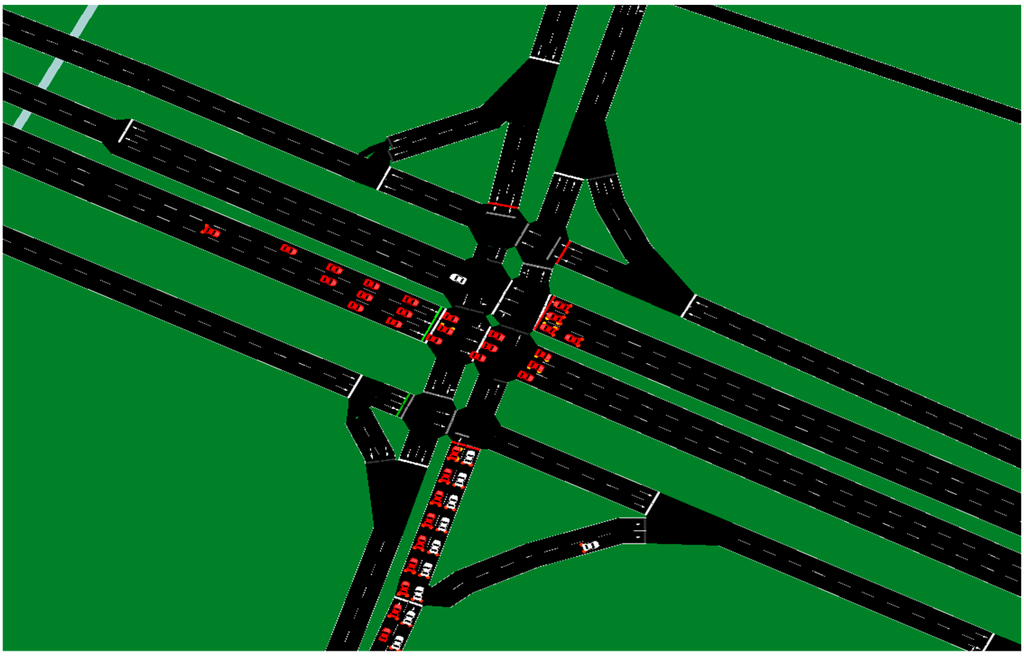
\includegraphics{sumo-simulator}
	\caption{Ejemplo de pantalla del simulador \gls{sumo}. Además de entorno de simulación propiamente dicho, \gls{sumo} provee de una interfaz gráfica que permite una visualización general, de zonas y de elementos en concreto a la vez que permite la variación de configuración de la simulación durante el desarrollo de la misma.}
	\label{fig:sumo-simulator}
\end{figure}

\begin{itemize}
	\item Multimodalidad permitiendo modelar no sólo tráfico de vehículos sino de peatones, bicicletas, trenes e incluso de barcos.
	\item Vehículos de diferentes tipologías, Simulación con y sin colisiones de vehículos.
	\item Diferentes tipos de vehículos y de carreteras, cada una con diferentes carriles y éstas con diferentes subdivisiones de subcarriles (diseño conceptual para permitir las simulaciones )
\end{itemize}

Al estar licenciado bajo la licencia \gls{gpl}, su distribución implica a su vez la distribución de su código fuente. Esto permite la modeificación de su comportamiento y el desarrollo de nuevos modelos integrados dentro del simulador. Sin embargo nosotros no haremos uso de esta característica, sino que usaremos \gls{sumo} como aplicación servidor y el módulo \gls{traci} como aplicación cliente desde donde gestionar todos los aspectos de cada simulación.

\subsection{La interfaz \glsentrylong{traci}}